\documentclass{beamer}
\usepackage{listings}
\lstset{
%language=C,
frame=single, 
breaklines=true,
columns=fullflexible
}
\usepackage{subcaption}
\usepackage{url}
\usepackage{tikz}
\usepackage{graphicx}
\usepackage{tkz-euclide} % loads  TikZ and tkz-base
%\usetkzobj{all}
\usetikzlibrary{calc,math}
\usepackage{float}
\usepackage{amsthm}
\usepackage{gensymb}
\newcommand\norm[1]{\left\lVert#1\right\rVert}
\renewcommand{\vec}[1]{\mathbf{#1}}
\newcommand{\R}{\mathbb{R}}
\newcommand{\C}{\mathbb{C}}
\newcommand{\comb}[2]{{}^{#1}\mathrm{C}_{#2}}
\providecommand{\brak}[1]{\ensuremath{\left(#1\right)}}
\providecommand{\abs}[1]{\vert#1\vert}
\providecommand{\fourier}{\overset{\mathcal{F}}{ \rightleftharpoons}}
\providecommand{\sbrak}[1]{\ensuremath{{}\left[#1\right]}}
\usepackage[export]{adjustbox}
\usepackage[utf8]{inputenc}
\usepackage{amsmath}
\DeclareMathOperator{\erfc}{erfc}
\usepackage[version=4]{mhchem}
\usetheme{Boadilla}
\title{Research Paper Presentation}
\author{Vikhyath Sai Kothamasu}
\institute{IITH}
\date{\today}
\begin{document}

\begin{frame}
\titlepage
\end{frame}
\begin{frame}{Title and Authors}
\begin{block}{Title}
Wide-band Channel Measurements and
Temporal-Spatial Analysis for Terahertz Indoor
Communications
\end{block}
\begin{block}{Authors}
\begin{enumerate}
    \item Ziming Yu, yuziming@huawei.com, Huawei Technologies Co., Ltd, China.
    \item Yi Chen, yidoucy@sjtu.edu.cn, Shanghai Jiao Tong University, China. 
    \item Guangjian Wang, wangguangjian@huawei.com, Huawei Technologies Co., Ltd, China.
    \item Weijun Gao, gaoweijun@sjtu.edu.cn, Shanghai Jiao Tong University, China. 
    \item Chong Han, chong.han@sjtu.edu.cn, Shanghai Jiao Tong University, China. 
\end{enumerate}
\end{block}
\end{frame}
\begin{frame}{Abstract}
\begin{enumerate}
    \item Terahertz communications are envisioned as a key technology for beyond 5G wireless systems, owing to its unprecedented multi-GHz bandwidth.
    \item A wide-band channel measurement between 130 GHz and 143 GHz is investigated in a typical meeting room.
    \item Physical parameters and insights in the THz indoor channel are comprehensively analyzed to find correlations among THz multipath
    characteristics.
\end{enumerate}
\end{frame}
\begin{frame}{Introduction}
\begin{enumerate}
    \item There has been an exponential growth in wireless data traffic recently which demands for high-speed wireless communication.
    \item The Terahertz (THz) (0.1-10 THz) band is capable of providing dozens and hundreds of gigahertz (GHz) continuous spectrum bands. Specifically, 140 GHz band is the first spectral window to penetrate into the THz band.
    \item One challenge is to measure, analyze, and model the THz electromagnetic wave propagation and channel characteristics.
\end{enumerate}
\end{frame}
\begin{frame}{Concepts}
\begin{block}{Bragg's Law}
Bragg's law provides the condition for a plane wave to be diffracted by a family of lattice planes: 
$$ 2d\sin \theta = n\lambda$$
where n is an integer representing order of reflection, $\lambda$ is the wavelength, d is the vector representing the displacement between reflection sites, $\theta$ is the angle between the reflected ray and the plane formed by the material's surface.
\\Waves reflected through an angle corresponding to n = 1 are said to be in the first order of reflection; the angle corresponding to n = 2 is the second order, and so on.
\end{block}
\end{frame}
\begin{frame}{Concepts}
\begin{block}{Complementary Error Function}
The complementary error function of x is defined as:
\begin{align}
    \erfc(x) &= \frac{2}{\sqrt{\pi}} \int_{x}^{\infty}e^{-t^2} \,dt
    \\ &= 1 - erf(x)
\end{align}
\end{block}
\end{frame}
\begin{frame}{Abbreviations}
\begin{center}
\begin{table}[h]
    \centering
    \scalebox{0.8}{
    \resizebox{\columnwidth}{!}{
\begin{tabular}{|c|c|}
\hline
\textbf{Abbreviation} & \textbf{Meaning} \\
\hline
THz & TeraHertz \\
\hline
Tx & Transmitter \\
\hline
Rx & Receiver \\
\hline
MPCs & Multi-Path Components \\
\hline
VNA & Vector Network Analyzer \\
\hline
HPBW & Half-Power BeamWidth \\
\hline
FSPL & Free Space Path Loss \\
\hline
LoS & Line of Sight \\
\hline
NLoS & Non Line of Sight \\
\hline
PDAP & Power-Delay-Angular Profiles \\
\hline
\end{tabular}
}
}
    \caption{Abbreviations used in presentation}
    \label{table 5}
\end{table}
\end{center}
\end{frame}


\begin{frame}{Experimental Setup}
\begin{enumerate}
    \item The experiment was conducted in a typical meeting room of dimensions 10.15 m × 7.9 m × 4 m.
    \item A 4.8 m × 1.9 m × 0.77 m desk is placed in the center, and a number of chairs are placed around the desk.
    \item Two TVs are closely placed and parallel to a wall.
    \item The material of one wall is glass, while the other three walls are lime walls.
    \item With a fixed Tx, multipath measurements are conducted at ten different receiver positions. Directional antennas are equipped at Tx and Rx to resolve MPCs in the angular domain.
\end{enumerate}
\end{frame}

\begin{frame}{Machinery Setup}
\begin{enumerate}
    \item The measurement platform consists of a 140 GHz transmission system and a VNA.
    \item The signal produced by VNA is up-converted to the frequency band from 130 to 140 GHz.
    \item The antennas at Tx and Rx are horn antennas.
    \item Tx produces an antenna gain of 15 dBi with the HPBW of $30\degree$ at 140 GHz.
    \item Rx produces an antenna gain of 25 dBi with the HPBW of $10\degree$ at 140 GHz.
    \item The two antennas are mounted on two rotation units and rotated by step motors, respectively.
\end{enumerate}
\end{frame}
\begin{frame}{Table of known parameters}
\begin{center}
\begin{table}[h]
    \centering
    \scalebox{0.65}{
    \resizebox{\columnwidth}{!}{
\begin{tabular}{|c|c|c|}
\hline
\textbf{Parameter} & \textbf{Symbol} & \textbf{Value} \\
\hline
Start frequency & $f_{start}$ & 130GHz \\ 
\hline
End frequency & $f_{end}$ & 140GHz \\ 
\hline
Bandwidth & $B_w$ & 13GHz \\
\hline
Sampling points & $N$ & 1301 \\
\hline
Sampling Interval & $\Delta f$ & 10MHz \\
\hline
Average noise floor & $P_N$ & -120 dBm \\
\hline
Test signal power & $P_{in}$ & 1mW \\
\hline
HPBW of transmitter & $HPBW^{Tx}$ & $30\degree$ \\
\hline
HPBW of receiver & $HPBW^{Rx}$ & $10\degree$ \\
\hline
Antenna gain at Tx & $G_t$ & 15dBi \\
\hline
Antenna gain at Rx & $G_r$ & 25dBi \\
\hline
Time domain resolution & $\Delta t$ & 76.9ps \\
\hline
Path length resolution & $\Delta L$ & 2.3cm \\
\hline
Maximum excess delay & $\tau_m$ & 100ns \\
\hline
Maximum path length & $L_m$ & 30m \\
\hline
\end{tabular}
}
}
    \caption{Known measurement parameters}
    \label{table 1}
\end{table}
\end{center}
\end{frame}
\begin{frame}{Image of setup}
\begin{figure}[!ht]
\centering
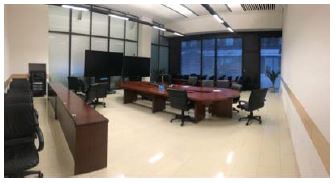
\includegraphics[width=0.7\columnwidth]{meeting room.JPG}
\caption{Meeting Room}
\label{image 1}
\end{figure}
\end{frame}
\begin{frame}{Image of setup plan}
\begin{figure}[!ht]
\centering
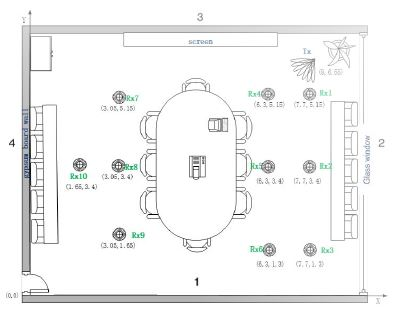
\includegraphics[width=0.7\columnwidth]{meeting layout.JPG}
\caption{Meeting Room Layout}
\label{image 2}
\end{figure}
\end{frame}
\begin{frame}{Calibration}
The S21 parameter for calibration, denoted by $S_{21}^{cal}$ is given by: 
$$S_{21}^{cal} = H_{sys}\times H_{att}$$
where $H_{att}$ is the channel transfer function of the THz attenuator which replaces the antennas connected to Tx and Rx; $H_{sys}$ is the channel transfer function of the measurement
system. The path loss of an LoS path is the negative number of its S21 parameter averaged over the measurement spectrum band.
The obtained values are then compared with the FSPL calculated by Friss' Law,
$$FSPL[dB] = -20\log_{10}\brak{\frac{c}{4\pi fd}}$$
where $c$ denotes the light speed, $f$ is the carrier frequency and $d$ is the separation distance between Tx and Rx.
\end{frame}
\begin{frame}{Calibration Results}
\begin{figure}[!ht]
\centering
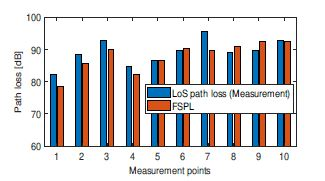
\includegraphics[width=0.7\columnwidth]{calibration.JPG}
\caption{Comparison between measured LoS path loss and FSPL}
\label{image 3}
\end{figure}
By comparison, we observe the measured path loss coincides with the FSPL computation having an average deviation of 2 dB indicating a successful calibration.
\end{frame}
\begin{frame}{Path Loss}
Path loss is defined as the transmit power divided by received power and is typically characterized in decibel scales as:
\begin{align}
    L = l_0 + 10n\log_{10}D + S
\end{align}
where $l_0$ is the path loss at a reference distance $d_0$ (typically 1m), n is the path loss exponent, D is the transmitter-receiver separation and S is the shadowing (noise), known as Log-normal, $S\sim N(0, \sigma_s^2)$.
\end{frame}
\begin{frame}{PDF of Path loss in a square region}
Let us normalize $L$ as: 
\begin{align}
    U = \frac{L-l_0}{\sigma_s} = \frac{10n\log_{10}D}{\sigma_s} + \frac{S}{\sigma_s}
\end{align}
Then, the normalized shadowing parameter is $\frac{S}{\sigma_s} \sim N(0,1)$. Let $(X_1, Y_1)$ and $(X_2, Y_2)$ represent a pair of transmitter and receiver. Then,
\begin{align}
    D &= \sqrt{(X_1-X_2)^2 + (Y_1-Y_2)^2}
    \\f_D(d) &= \begin{cases}
    \frac{2d^3}{a^4} + \frac{8d^2}{a^3} + \frac{2\pi d}{a^2} & 0\leq d<a\\ ~\\[-1em]
    -\frac{2d^3}{a^4}+ \brak{-\frac{4}{a^2} + \frac{8\arcsin(\frac{a}{d})}{a^2}+\frac{8\sqrt{d^2-a^2}}{a^3}-\frac{2\pi}{a^2}} & a\leq d \leq \sqrt{2}a
        \end{cases}
    \\&\approx \begin{cases}
    \frac{2d^3}{a^4} + \frac{8d^2}{a^3} + \frac{2\pi d}{a^2} & 0\leq d<a\\ ~\\[-1em]
    \frac{-8(d-\sqrt{2}a)^3}{3a^4} & a\leq d \leq \sqrt{2}a
    \end{cases} \label{equation 1}
\end{align}
\end{frame}
\begin{frame}{PDFs}
Let   
\begin{align}
    Y = \frac{10n\log_{10}(D)}{\sigma_s}
\end{align}
Then, the PDF of Y can be transformed from equation \eqref{equation 1} as
\begin{align}
    f_Y(y) = \begin{cases}
    \frac{2\xi e^{4\xi y}}{a^4} - \frac{8\xi e^{3\xi y}}{a^3} + \frac{2\pi \xi e^{2\xi }}{a^2} & -\infty < y < \frac{\ln{a}}{\xi}\\ ~\\[-1em]
    -\frac{8\xi e^{4\xi y}}{3a^4}+ \frac{8\sqrt{2}\xi e^{3\xi y}}{a^3} - \frac{16\xi e^{2\xi y}}{a^2} + \frac{16\sqrt{2}\xi e^{\xi y}}{3a} & \frac{\ln{a}}{\xi} \leq y \leq \frac{\ln{(\sqrt{2}a)}}{\xi}
        \end{cases}
\end{align}
where $\xi = \frac{\ln{(10)}\sigma_s}{10n}$. 
\end{frame}
\begin{frame}{PDF of U}
Furthermore, as S and D are independent, the PDF of U is the convolution integration of $f_Y(y)$ with the Gaussian normal function:
\begin{align}
    f_U(u) = \int_{-\infty}^{\infty}f_Y(y)\frac{1}{\sqrt{2}\pi}\exp{\brak{-\frac{(u-y)^2}{2}}} \,dy
\end{align}
\begin{multline}
    f_U(u) = \brak{\frac{\xi \pi e^{2\xi u + 2\xi^2}}{a^2} - \frac{4\xi e^{3\xi u + \frac{9}{2}\xi^2}}{a^3} + \frac{\xi e^{4\xi u+8\xi^2}}{a^4}} \times 
    \\\erfc\brak{\frac{\xi u-\ln{a} + 2\xi^2}{\sqrt{2}\xi}} 
    \\ +\brak{\erfc\brak{\frac{\xi u-\ln{(\sqrt{2}a)} + 2\xi^2}{\sqrt{2}\xi}} 
    - \erfc \brak{\frac{\xi u-\ln{a} + 2\xi^2}{\sqrt{2}\xi}}} \times 
    \\ \brak{-\frac{4\xi e^{4\xi u + 8\xi ^2}}{3a^4} + \frac{4\sqrt{2}\xi e^{3\xi u + \frac{9}{2}\xi^2}}{a^3} - \frac{8\xi e^{2\xi u +2\xi^2}}{a^2} + \frac{8\sqrt{2}\xi e^{\xi u + \frac{1}{2}\xi^2}}{3a}} \label{equation 2}
\end{multline}
for $u\leq \frac{\ln{(\sqrt{2}a)}}{\xi} + 3$ where $\erfc(.)$ is the complementary error function.
\end{frame}
\begin{frame}{PDF and CDF of L}
Finally, the PDF of L is transformed from equation \eqref{equation 2} as:
\begin{align}
    f_L(l) = \frac{1}{\sigma_s}f_U\brak{\frac{l-l_0}{\sigma_s}}
\end{align}
for $l\leq l_0 + \frac{\sigma_s\ln{(\sqrt{2}a)}}{\xi} + 3\sigma_s$. The CDF can also be explicitly given, but the resulting formula is too lengthy and complex. Instead, the CDF when plotted for discrete values looks like: 
\begin{figure}[!ht]
\centering
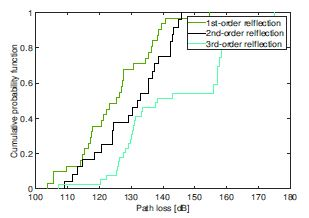
\includegraphics[width=0.4\columnwidth]{cdf.JPG}
\caption{CDF of reflected paths}
\label{image 4}
\end{figure}
\end{frame}
\begin{frame}{Reflection List}
\begin{center}
\begin{table}[h]
    \centering
    \scalebox{0.9}{
    \resizebox{\columnwidth}{!}{
\begin{tabular}{|c|c|c|c|c|c|c|c|c|}
\hline
\multicolumn{1}{|c|}{RX} & \multicolumn{1}{c|}{Number of MPCs} & \multicolumn{2}{c|}{1st-order reflection} & \multicolumn{2}{c|}{2nd-order reflection} & \multicolumn{2}{c|}{3rd-order reflection} & \multicolumn{1}{c|}{$\frac{P_{Wall}}{P_{Obstacle}}$} \\
\cline{3-8}
\multicolumn{1}{|c|}{} & \multicolumn{1}{|c|}{} & Wall & Obstacle & Wall & Obstacle & Wall & Obstacle & \multicolumn{1}{|c|}{} \\
\hline
1 & 8 & 1 & 3 & 2 & 0 & 2 & 0 & 1.10 \\
\hline
2 & 11 & 3 & 1 & 4 & 1 & 2 & 0 & 9.08 \\
\hline
3 & 11 & 3 & 3 & 4 & 0 & 1 & 0 & 9.08 \\
\hline
4 & 14 & 3 & 3 & 3 & 1 & 3 & 1 & 8.14 \\
\hline
6 & 8 & 3 & 0 & 3 & 0 & 1 & 1 & 618.65 \\
\hline
7 & 8 & 2 & 0 & 2 & 0 & 2 & 2 & 13.13 \\
\hline
8 & 6 & 2 & 0 & 1 & 1 & 2 & 0 & 9.58 \\ 
\hline
9 & 5 & 2 & 0 & 1 & 0 & 2 & 0 & $\inf$ \\
\hline
10 & 5 & 2 & 0 & 1 & 0 & 0 & 2 & 0.95 \\
\hline
\end{tabular}
}
}
    \caption{Reflections of MPCs for all the receivers}
    \label{table 2}
\end{table}
\end{center}  
\end{frame}
\begin{frame}{Multipath PDAPs}
\begin{figure}[!ht]
\centering
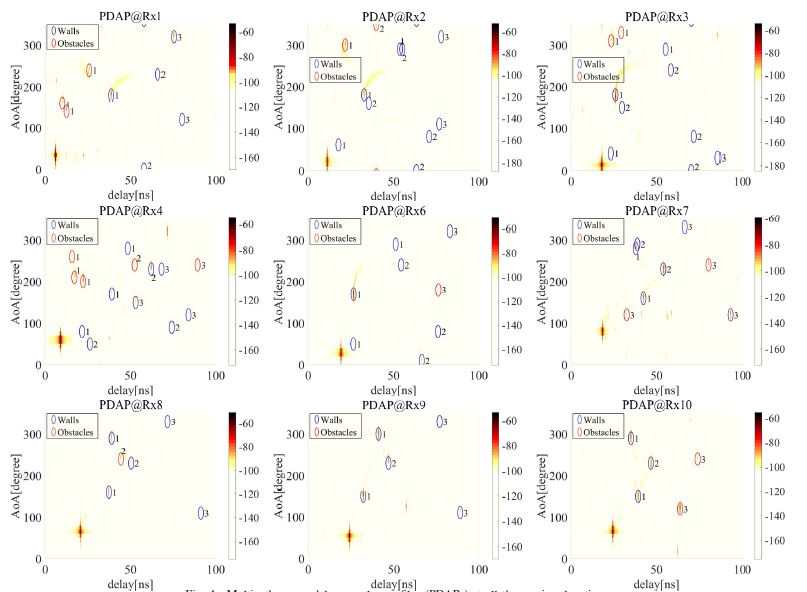
\includegraphics[width=0.8\columnwidth]{pdaps.JPG}
\caption{Multipath PDAPs at all receivers}
\label{image 5}
\end{figure}   
\end{frame}
\begin{frame}{Temporal and Spatial features}
\begin{enumerate}
    \item K-factor: Defined as the ratio between the power of the LoS path and the power of the remaining NLoS MPCs.
    \item RMS Delayspread (DS) = 
    \begin{align}
        \tau_{rms} &= \sqrt{\brak{\frac{\int_{0}^{\infty}(\tau-\overline{\tau})^2A_c(\tau) \,d\tau}{\int_{0}^{\infty}A_c(\tau) \,d\tau}}}
        \\ \text{with } \overline{\tau} &= \frac{\int_{0}^{\infty}\tau A_c(\tau) \,d\tau}{\int_{0}^{\infty} A_c(\tau) \,d\tau}
    \end{align}
    where $A_c(\tau)$ denotes the power angular profile.
    \item Angular spread (AS) can be modelled as: 
    \begin{align}
        \sigma_{\varphi/\theta}(d^2) = a\times d^2 + bd + c + \chi_{\sigma}
    \end{align}
    where $\chi_{\sigma}$ denotes a zero mean Gaussian random variable with the standard deviation $\sigma$, accounting for the deviations of the individual spreads from the polynomial function.
\end{enumerate}
\end{frame}
\begin{frame}{Statistics}
\begin{center}
\begin{table}[h]
    \centering
    \scalebox{0.65}{
    \resizebox{\columnwidth}{!}{
\begin{tabular}{|c|c|c|c|c|}
\hline
RX & Distance [m] & K-factor [dB] & DS [ns] & AS [$\degree$] \\
\hline
1 & 1.43 & 39.57 & 3.58 & 25.23 \\
\hline
2 & 3.16 & 29.07 & 1.9 & 20.45 \\
\hline
3 & 5.26 & 26.14 & 2.95 & 33.97 \\
\hline
4 & 2.20 & 26.65 & 5.72 & 20.95 \\
\hline
6 & 5.52 & 15.96 & 1.17 & 26.27 \\
\hline
7 & 5.14 & 20.07 & 10.02 & 39.23 \\
\hline
8 & 5.87 & 20.38 & 1.62 & 16.67 \\
\hline
9 & 6.97 & 12.60 & 3.95 & 29.12 \\
\hline
10 & 7.12 & 12.40 & 5.87 & 31.54 \\
\hline
\end{tabular}
}
}
    \caption{Statistics of MPCs for each receiver}
    \label{table 3}
\end{table}
\end{center}
\end{frame}
\begin{frame}{Correlation Matrix}
A correlation matrix is a table showing correlation coefficients between variables. Each cell in the table shows the correlation between two variables.
Let $r_{jk}$ be the correlation coefficient between variables $x_j$ and $x_k$.
\begin{align}
    r_{jk} &= \frac{\Sigma_{i=1}^{n}(x_{ij} - \overline{x_{j}})(x_{ik} - \overline{x_{{k}}})}{\sqrt{\Sigma_{i=1}^{n}(x_{ij} - \overline{x_{j}})^2}\sqrt{\Sigma_{i=1}^{n}(x_{ik} - \overline{x_{k}})^2} }
    \\Cor(x_j, x_k) &= \frac{\Sigma_{i=1}^{n}(x_{ij} - \overline{x_{j}})(x_{ik} - \overline{x_{{k}}})}{\sqrt{\Sigma_{i=1}^{n}(x_{ij} - \overline{x_{j}})^2}\sqrt{\Sigma_{i=1}^{n}(x_{ik} - \overline{x_{k}})^2} }
    \\ &= \begin{cases}
    1 & \text{if } j=k\\ ~\\[-1em]
    r_{jk} & \text{if } j\neq k
        \end{cases}
\end{align}
\end{frame}
\begin{frame}{Correlation Matrix}
The correlation matrix for the characteristics is:
\begin{center}
\begin{table}[h]
    \centering
    \scalebox{0.9}{
    \resizebox{\columnwidth}{!}{
\begin{tabular}{|c|c|c|c|c|c|c|}
\hline
 & d & N & K & DS & AS & $\frac{P_{Wall}}{P_{Obstacle}}$ \\
\hline
Distance & 1.00 & - & - & - & - & - \\
\hline
Number of MPCs & -0.70 & 1.00 & - & - & - & - \\
\hline
K-factor & -0.67 & 0.02 & 1.00 & - & - & - \\
\hline
Delay Spread & 0.04 & 0.00 & -0.09 & 1.00 & - & - \\
\hline
Angular Spread & 0.37 & -0.20 & -0.13 & 0.66 & 1.00 & - \\
\hline
$\frac{P_{Wall}}{P_{Obstacle}}$ & 0.41 & -0.42 & -0.15 & -0.02 & 0.11 & 1.00 \\
\hline
\end{tabular}
}
}
    \caption{Correlation matrix among THz multipath characteristics}
    \label{table 4}
\end{table}
\end{center}
\end{frame}
\begin{frame}{Conclusions}
\begin{enumerate}
    \item The THz indoor channel is sparse in both temporal and spatial domains, while the number of MPCs is less than 10.
    \item Although the transmitter directs a narrow beam to the receiver, the existence of MPCs is still not negligible, especially when receivers are far from Tx.
    \item Wall-reflected MPCs contain considerably higher power than other obstacle-reflected MPCs in THz indoor environment.
    \item A longer communication distance might cause a high sparsity, smaller K-factor, broader angular spread, and stronger wall-reflected power.
\end{enumerate}
\end{frame}
\end{document}
